\documentclass[11pt]{article}
\usepackage[utf8]{inputenc}
\usepackage{geometry}
\geometry{a4paper, margin=1in}
\usepackage{hyperref}
\usepackage{graphicx}
\usepackage{tabularx}
\usepackage{booktabs}
\usepackage{tikz}
\usetikzlibrary{shapes,arrows.meta,positioning,fit,backgrounds}

\title{Landslide Identification — Test Results \\ \large EfficientNet-B3 Transfer Learning (results2)}
\author{}
\date{2026-03-12}

\begin{document}

\maketitle

\noindent\textbf{GPU:} NVIDIA RTX 2000 Ada Generation \\
\textbf{Environment:} conda landslide-ml (PyTorch cu124, Python 3.10) \\

\section{Improvements Implemented}

\begin{enumerate}
    \item \textbf{More powerful architecture — EfficientNet-B3} \\
          Replaced AlexNet with EfficientNet-B3 (300x300 input, 1536-dim feature head). Feature layers were frozen for the first 5 epochs to preserve ImageNet embeddings, and fully unfrozen at epoch 6 with differential learning rates (head: 1e-4, features: 1e-5). EfficientNet-B3 relies on compound scaling (depth, width, resolution), offering superior feature extraction compared to AlexNet despite having fewer parameters ($\sim$12M vs $\sim$62M).
    \item \textbf{Input Resolution Upgrade} \\
          The input tensor was scaled from 227x227 up to 300x300. This is the native resolution for EfficientNet-B3 and allows the network to process finer textural details (like small rock distributions).
    \item \textbf{CosineAnnealingLR Scheduler} \\
          We implemented a smooth learning rate decay instead of the hard StepLR drops used in the baseline.
\end{enumerate}

\section{Architecture Flowchart}
\begin{center}
    \resizebox{0.9\textwidth}{!}{
    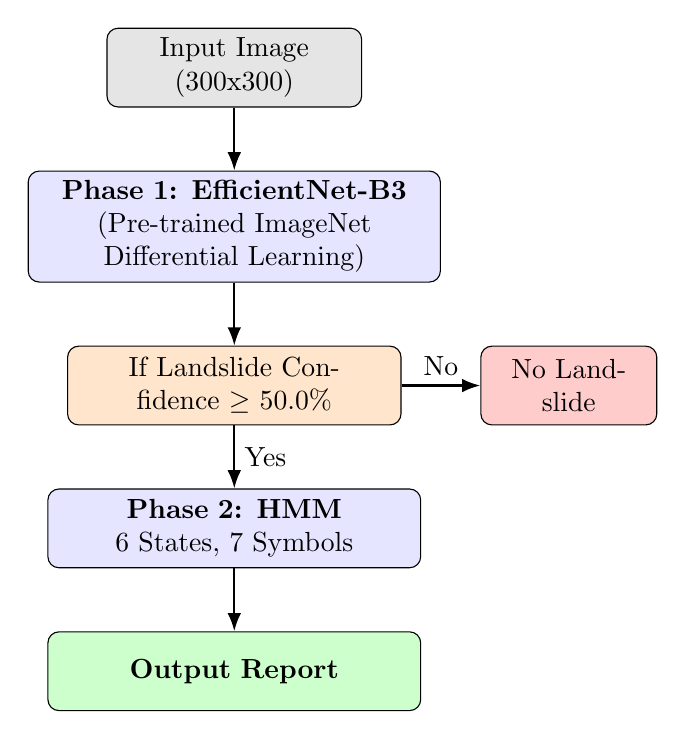
\begin{tikzpicture}[
        node distance=0.8cm and 1cm,
        box/.style={draw, rectangle, rounded corners, align=center, fill=blue!10, text width=3cm, minimum height=1cm},
        arrow/.style={-Latex, thick}
    ]
        % Inputs
        \node[box, fill=gray!20] (input) {Input Image (300x300)};
        
        % Phase 1
        \node[box, below=of input, text width=5cm] (phase1) {\textbf{Phase 1: EfficientNet-B3}\\(Pre-trained ImageNet\\ Differential Learning)};
        \node[box, below=of phase1, fill=orange!20, text width=4cm] (decision) {If Landslide Confidence $\ge$ 50.0\%};
        
        % Phase 2
        \node[box, below=of decision, text width=4.5cm] (phase2) {\textbf{Phase 2: HMM}\\6 States, 7 Symbols};
        
        % Outputs
        \node[box, below=of phase2, fill=green!20, text width=4.5cm] (output) {\textbf{Output Report}};
        
        % Connections
        \draw[arrow] (input) -- (phase1);
        \draw[arrow] (phase1) -- (decision);
        \draw[arrow] (decision) -- node[right] {Yes} (phase2);
        \draw[arrow] (phase2) -- (output);
        
        % No branch
        \node[box, right=of decision, fill=red!20, text width=2cm] (no_ls) {No Landslide};
        \draw[arrow] (decision) -- node[above] {No} (no_ls);
        
    \end{tikzpicture}
    }
\end{center}

\section{Phase 1 — Full Test Set Evaluation}

\noindent \textbf{Test set:} 699 images (211 landslide + 488 non\_landslide) \\
\textbf{Checkpoint:} checkpoints/efficientnet\_b3\_best.pth (epoch 24, val\_acc=79.82\%) \\

\vspace{0.3cm}
\begin{table}[h]
    \centering
    \begin{tabular}{@{}ll@{}}
        \toprule
        \textbf{Metric} & \textbf{Score} \\ \midrule
        Accuracy & 79.97\% \\
        Precision & 63.71\% \\
        Recall & 78.20\% \\
        F1-Score & 70.21\% \\
        ROC-AUC & 88.93\% \\ \bottomrule
    \end{tabular}
\end{table}

\subsection{Confusion Matrix}
\begin{table}[h]
    \centering
    \begin{tabular}{@{}lcc@{}}
        \toprule
        & \textbf{Predicted: non\_landslide} & \textbf{Predicted: landslide} \\ \midrule
        \textbf{Actual: non\_landslide} & 394 & 94 \\
        \textbf{Actual: landslide} & 46 & 165 \\ \bottomrule
    \end{tabular}
\end{table}

\textbf{Analysis:} EfficientNet-B3 significantly improves Recall (+9.95\%) and F1-Score (+2.76\%) over pretrained AlexNet (results1.md). Precision is slightly lower — the model detects more true landslides but also more false positives. For disaster monitoring, high recall is deliberately favored over precision.

\end{document}
